\subsection{ISAtoSA}
\label{isa2sa}
Einige der im Framework enthaltenden Algorithmen, wie beispielsweise der mSufSort oder der qSufSort, konstruieren anstelle des eigentlichen Suffix-Arrays stattdessen die inverse Permutation, das inverse Suffix-Array. \\
\begin{definition}[Inverses Suffix-Array]
Das Inverse Suffix-Array, kurz $\mathsf{ISA}$, bezeichnet ein Array, in dem zu jedem
Suffix sein lexikographischer Rang gespeichert wird, der seiner Position
im Suffix-Array entspricht.\\
Es gilt also $\mathsf{ISA}[\mathsf{SA}[i]]=i.$
%, falls $\mathsf{ISA}$[$i$] = $j$, dann $\mathsf{SA}$[$j$] = $i$.
\end{definition}
Um daraus das $\mathsf{SA}$ konstruieren zu können, wurden innerhalb des Frameworks drei unterschiedliche Ansätze implementiert, die wir im Folgenden vorstellen werden.
\subsubsection{Simple Scan}
Wie der Titel andeutet, handelt es sich bei dieser Variante um den straight-forward Ansatz, der über die Indizes iteriert und die Einträge im $\mathsf{SA}$ wie folgt überschreibt:
\begin{equation}
\mathsf{SA}[\mathsf{ISA}[i]]=i, \text{ für } 0\leq i < n
\end{equation}

Voraussetzung für diese Methode ist, dass der Speicherplatz für sowohl das $\mathsf{SA}$, als auch das $\mathsf{ISA}$ bereits verfügbar ist. Nachteil dieser Methode ist es, dass viele zufällige Sprünge innerhalb des Suffix-Arrays gemacht werden, worunter die Cache-Effizienz leidet. 
\subsubsection{Inplace Scan}
Im Fall, dass ausschließlich Speicher für das $\mathsf{ISA}$ zur Verfügung steht, eignet sich der Simple Scan nicht, da dafür zusätzlicher Speicher für ein Array der Länge des Textes allokiert werden müsste. Daher wurde darüber hinaus eine Variante implementiert, die \textit{inplace} arbeitet, also ausschließlich das gegebene $\mathsf{ISA}$ Array nutzt und darin auch das Ergebnis speichert \cite{saca:8}. Voraussetzung dafür ist, dass die Ränge im vorliegenden $\mathsf{ISA}$ kleiner $0$ sind.\\
Die Idee ist, es zyklisch die Ränge im $\mathsf{ISA}$ durch die Positionen im $\mathsf{SA}$ zu ersetzen. Angenommen, wir finden Rang $r = \mathsf{SA}[s]$. Nun überschreiben wir $\mathsf{ISA}[r-1]=r$ merken uns aber den vorherigen Inhalt, um nach dem Überschreiben weiter dahin springen zu können. Auf diese Weise durchlaufen wir das Array bis jeder Rang durch einen $\mathsf{SA}$-Index ersetzt wurde.\\
Vorteil dieser Methode ist, wie bereits erwähnt, dass kein zusätzlicher Speicherplatz für das Ergebnisarray benötigt wird. Der allerdings weiterhin bestehende Nachteil ist, dass viele zufällige, cache-unfreundliche Sprünge gemacht werden. Zudem wird das letzte Bit zur Unterscheidung zwischen Rängen und Indizes benötigt, wodurch der Wertebereich eingeschränkt wird.
\subsubsection{Multi Scan}
Die Multi Scan Variante von Maniscalco und Puglisi \cite{saca:8} soll im Gegensatz zu den beiden vorherigen Methoden cache-freundlich arbeiten und dabei weniger zusätzlichen Speicher benötigen als die \textit{Simple Scan} Variante.\\
Wir definieren $Q_i$ mit $i \in \{1,2,3,4\}$, als $i$-tes Viertel des $\mathsf{SA}$. Zu Beginn des Algorithmus werden zwei zusätzliche Arrays $x_a$ und $x_b$ mit jeweils der Größe $\frac{n}{4}$ angelegt. In der ersten Phase wird das $\mathsf{ISA}$ von links nach rechts durchlaufen und falls ein Rang $r$ aus $Q_1$ gefunden wurde, wird dieses an die Stelle $x_a[r]$ verschoben und seine Position in $\mathsf{ISA}$ als leer markiert. Nach Abschluss der ersten Phase liegt $Q_1$ sortiert in $x_a$.\\
In der zweiten Phase scannen wir das $\mathsf{ISA}$ erneut von links nach rechts. Finden wir nun einen Rang $r \in Q_2$ speichern wir diesen an der jeweiligen Position in $x_b$ und markieren auch hier die Position in $\mathsf{ISA}$ als leer. An jede leere Position die wir während des Scans finden oder erzeugen, verschieben wir die erste besetze Position aus $x_a$ und markieren ihre Zugehörigkeit zu $Q_1$ mit Hilfe eines Bit-Tags. \\
Die dritte und vierte Phase laufen analog ab. Wir durchlaufen also das $\mathsf{ISA}$ und verschieben die jeweiligen Ränge aus $Q_i$ in das zu dem Zeitpunkt freie Hilfsarray. \\
Nach Ablauf der vierten Phase haben wir also die Ränge aus $Q_4$ in $x_b$ gespeichert und $\frac{n}{4}$ freie Stellen am Ende des $\mathsf{ISA}$ Arrays. Wir kopieren $x_b$ ans Ende von $\mathsf{ISA}$, wodurch die Elemente aus $Q_4$ dann an der richtigen Stelle stehen und nicht weiter beachtet werden müssen.\\
In der nächsten Phase müssen dann also ausschließlich die Ränge aus $Q_1,Q_2$ und $Q_3$ in die richtige Reihenfolge gebracht werden. Dazu scannen wir erneut das $\mathsf{ISA}$ Array von links nach rechts bis wir die Position $\frac{3n}{4}-1$ erreichen. Finden wir dabei ein Element aus $Q_2$, verschieben wir dieses nach $x_a$ und Elemente aus $Q_3$ nach $x_b$. Ränge aus $Q_1$ werden dabei an die erste freie Position in $\mathsf{ISA}$ verschoben. Die Zugehörigkeit eines Ranges lässt sich dabei anhand des Tags feststellen. Zum Ende des Scans haben wir dann also $Q_1$ am Anfang des $\mathsf{ISA}$, $Q_2$ in $x_a$ und $Q_3$ in $x_b$. \\
In der letzten Phase wird dann $x_a$ nach $\mathsf{ISA}[\frac{n}{4},...,\frac{n}{2}-1]$ und $x_b$ nach \\ $\mathsf{ISA}[\frac{n}{2},...,\frac{3n}{4}-1]$ verschoben. Wir erhalten also an dieser Stelle das fertige $\mathsf{SA}$ Array. EIn Beispiel für diese Variante zeigt Abb. $\ref{multiscan}$\\
Auch wenn bei dieser Variante deutlich mehr Durchläufe durch das $\mathsf{ISA}$ Array gemacht werden, behaupten die Autoren, dass dadurch das es sich dabei lediglich um cache-freundliche Scans von links nach rechts handelt, Laufzeit im Gegensatz zu den cache-unfreundlichen Varianten gewinnen zu können. Nachteile dieser Variante sind jedoch zum einen die höhere Komplexität im Vergleich zu den beiden vorherigen Varianten und zum anderen, dass hierbei die drei MSB für Tags benötigt werden, wodurch hier, noch mehr als bei der inplace Variante, der Wertebereich eingeschränkt wird.
\begin{center}
\begin{figure}
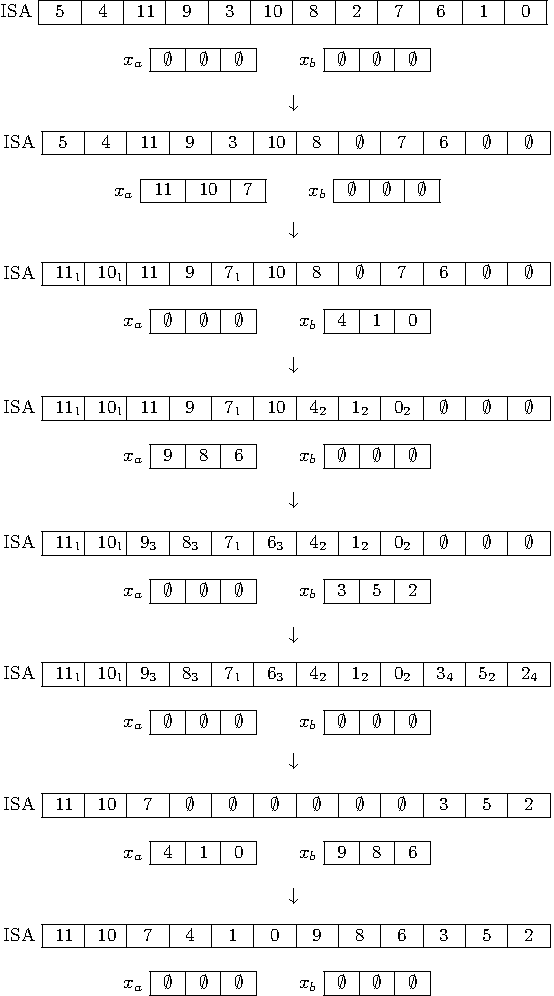
\includegraphics[scale=1]{kapitel/4_komponenten/techniken/bilder/MultiScanExample.pdf}
\caption{Beispiel für den ISAtoSA Multi Scan anhand des $\mathsf{ISA}$ für den Text $\mathsf{T}=MISSISSIPI\$$.}
\label{multiscan}
\end{figure}
\end{center}
